\subsection{El circuito}
\begin{figure}[H]
    \centering
    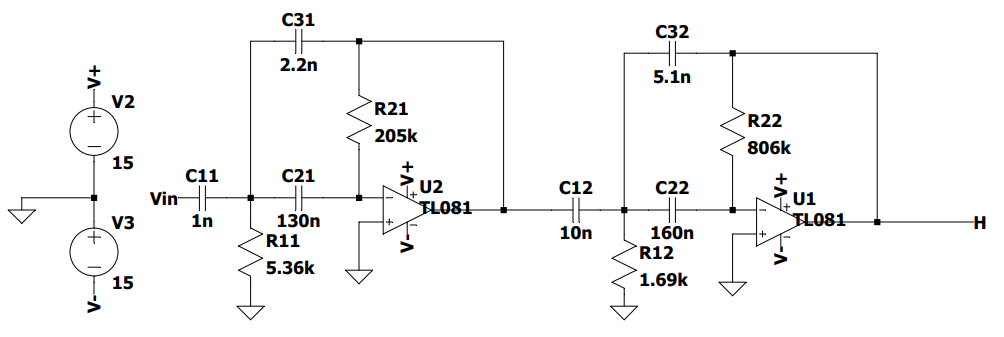
\includegraphics[width=1\textwidth]{resources/Circuito.PNG}
    \caption{Implementación del circuito en LTSpice}
\end{figure}

\subsection{Diagramas de Bode}
\begin{figure}[H]
    \centering
    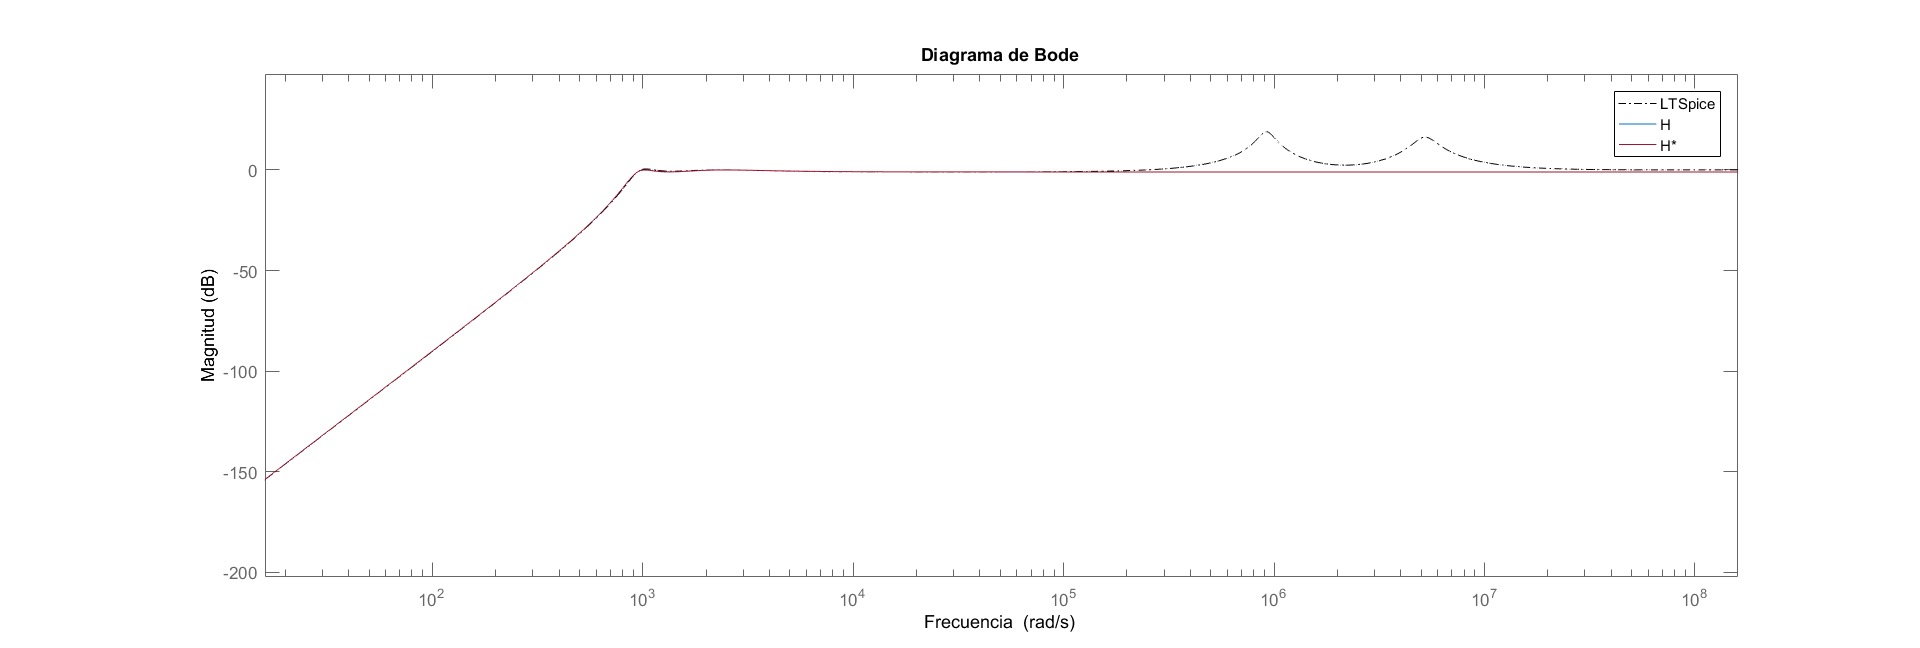
\includegraphics[width=1\textwidth]{resources/Bode_LTSpice.png}
    \caption{Diagrama de magnitud de Bode}
\end{figure}

\begin{figure}[H]
    \centering
    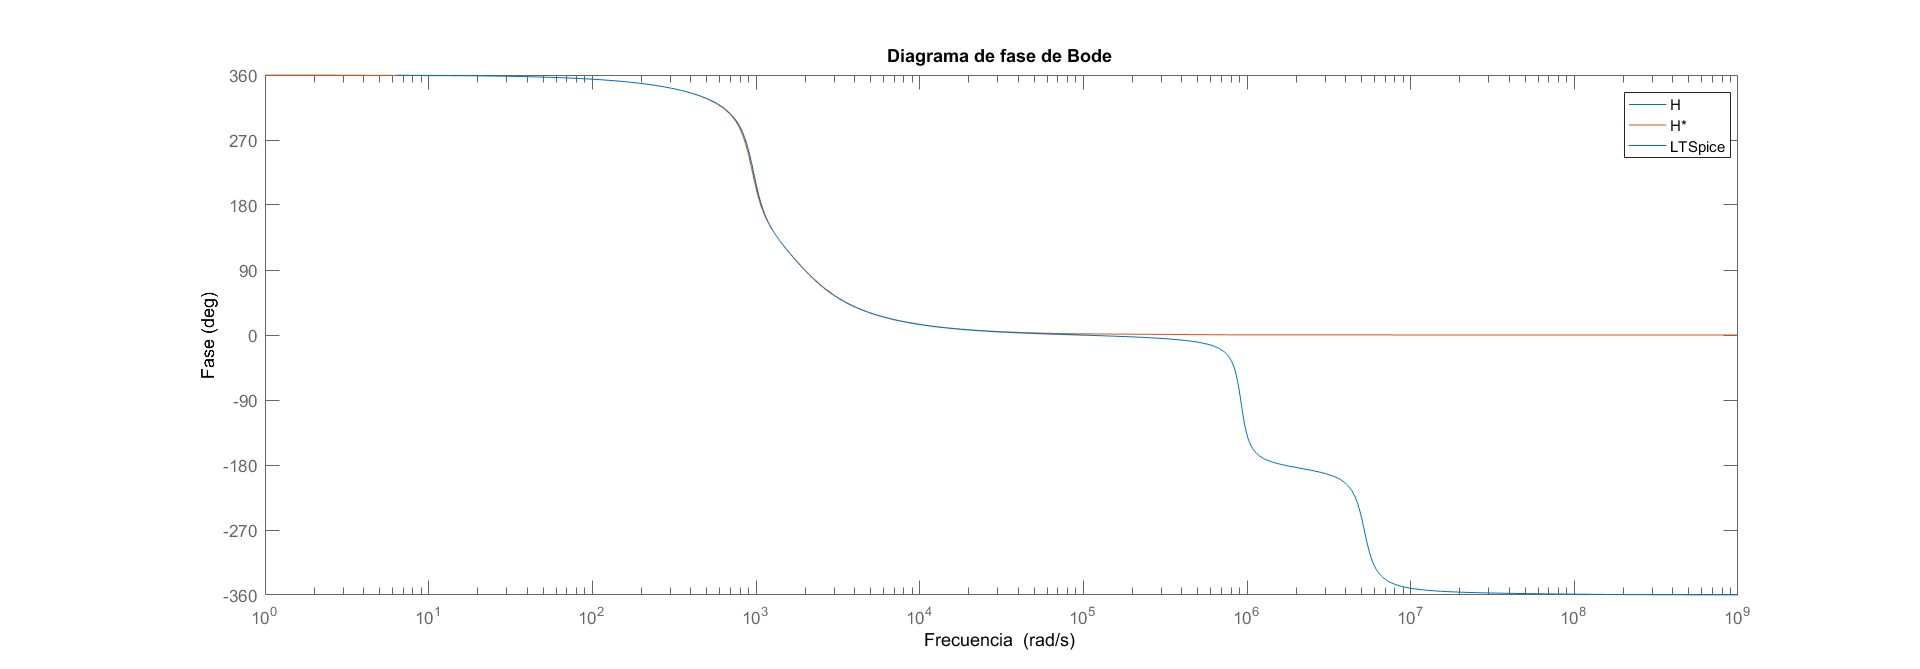
\includegraphics[width=1\textwidth]{resources/BodeFase_LTSpice.png}
    \caption{Diagrama de fase de Bode}
\end{figure}

En estos gráfico podemos ver que, a diferencia de los anteriores gráficos, aquí se puede percibir una diferencia a altas frecuencias entre lo obtenido con las simulaciones matemáticas en MatLab y lo obtenido en la simulación circuital en LTSpice. Esto se puede explicar con el uso de un modelo real para el amplificador operacional, el cual a altas frecuencias introduce nuevas singularidades al circuito que generan una diferencia en el diagrama de Bode esperado.

\subsection{Respuesta al escalón}
\begin{figure}[H]
    \centering
    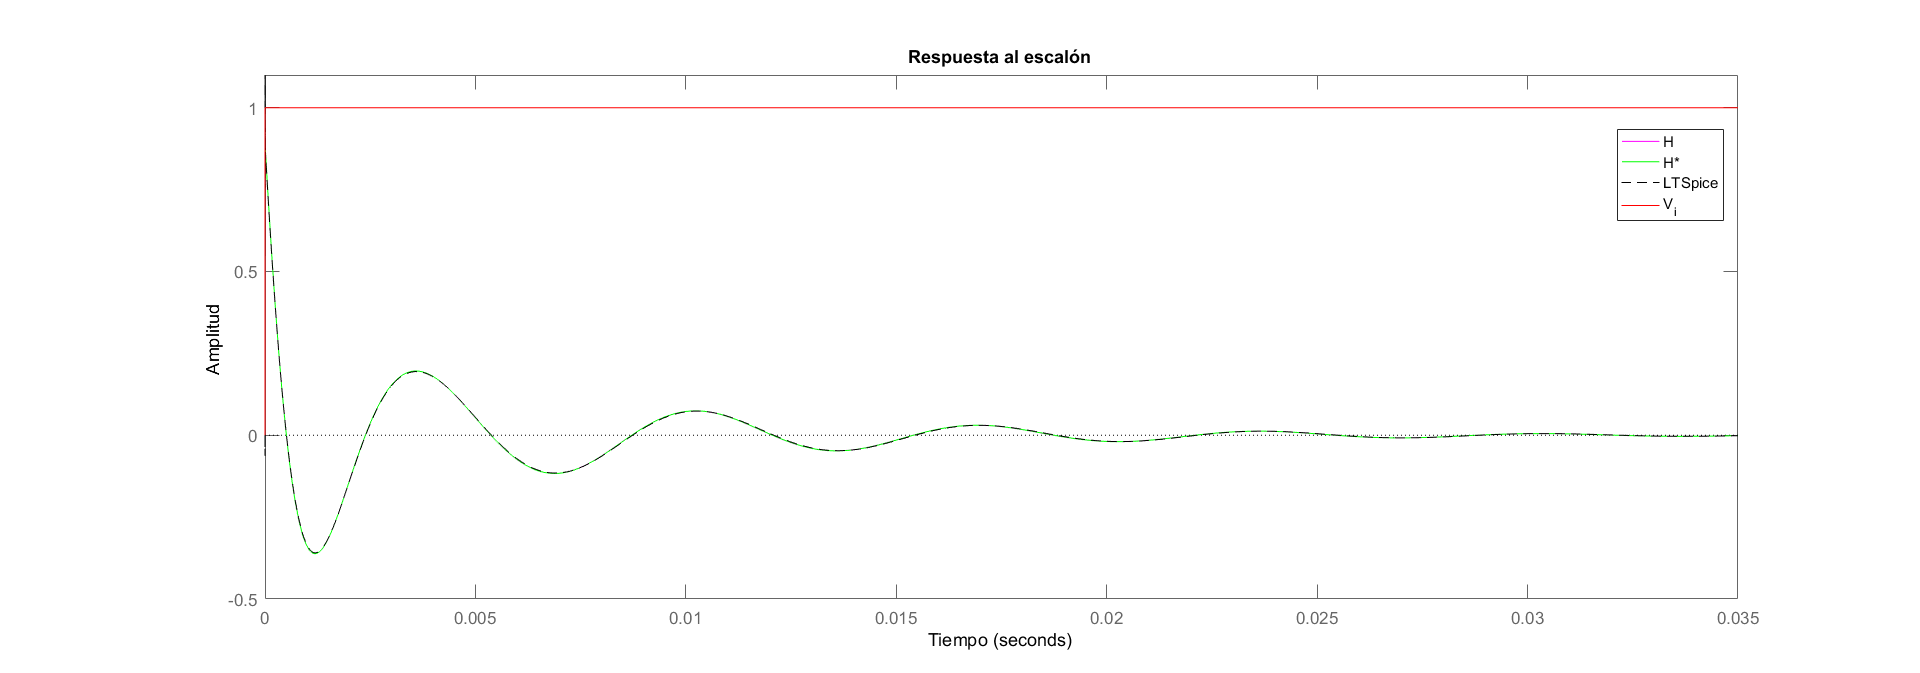
\includegraphics[width=1\textwidth]{resources/Escalon_LTSpice.png}
    \caption{Respuesta al escalón}
\end{figure}

Podemos ver en este gráfico que la señal de salida simulada con el circuito de LTSpice con el amplificador ideal es prácticamente la misma que la salida con la simulación numérica.

\subsection{Respuesta a la señal senoidal}
\begin{figure}[H]
    \centering
    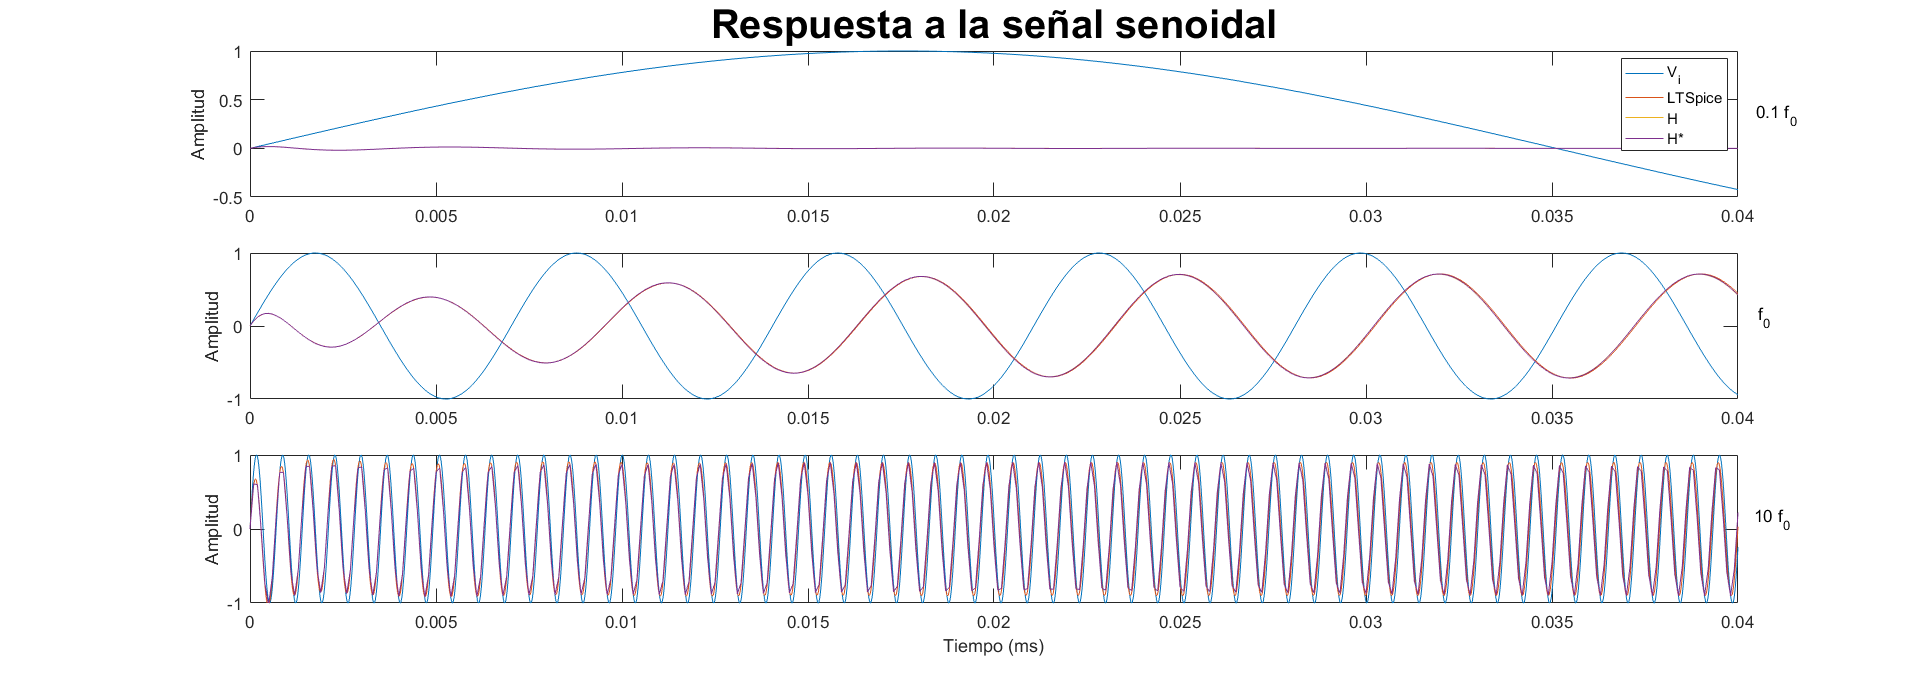
\includegraphics[width=1\textwidth]{resources/Comparacion_senoidal_LT.png}
    \caption{Respuesta a la señal senoidal}
\end{figure}
En los primeros dos gráficos no hay una difernecia significativa entre la señal de salida simulada matemáticamente y la señal de salida simulada por LTSpice con el amplificador operacional. Luego, para el tercer gráfico podemos ver que sí existe una diferencia, sobre todo en las puntas, para las señales de salida, siendo que para la salida simulada con LTSpice se obtiene una mayor ganancia que para la esperada matemáticamente. Esto podría deberse a múltiples factores.
El primer factor podría ser una discretización de la señal de salida obtenida con MatLab ya que se nota que en las puntas no parecen haber cambios suaves, sino más bien puntiagudos, y esto podría deberse a falta de muestreo por el software utilizado.
El segundo factor podría ser la alta frecuencia de la señal de entrada, como ya hemos visto en el diagrama de Bode para la magnitud, para frecuencias muy altas el circuito comienza a comportarse de forma diferente a la esperada matemáticamente ya que este modelo (el matemático) no tiene en cuenta el circuito interno del amplificador operacional real, mientras que LTSpice sí lo tiene en cuenta, de todas formas no es factible que el problema sea debido a esto último comentado, ya que para llegar a diferencias significativas la frecuencia debe ser, al menos, 2 órdenes de magnitud superior.

\subsection{Respuesta a la señal cuadrada}
\begin{figure}[H]
    \centering
    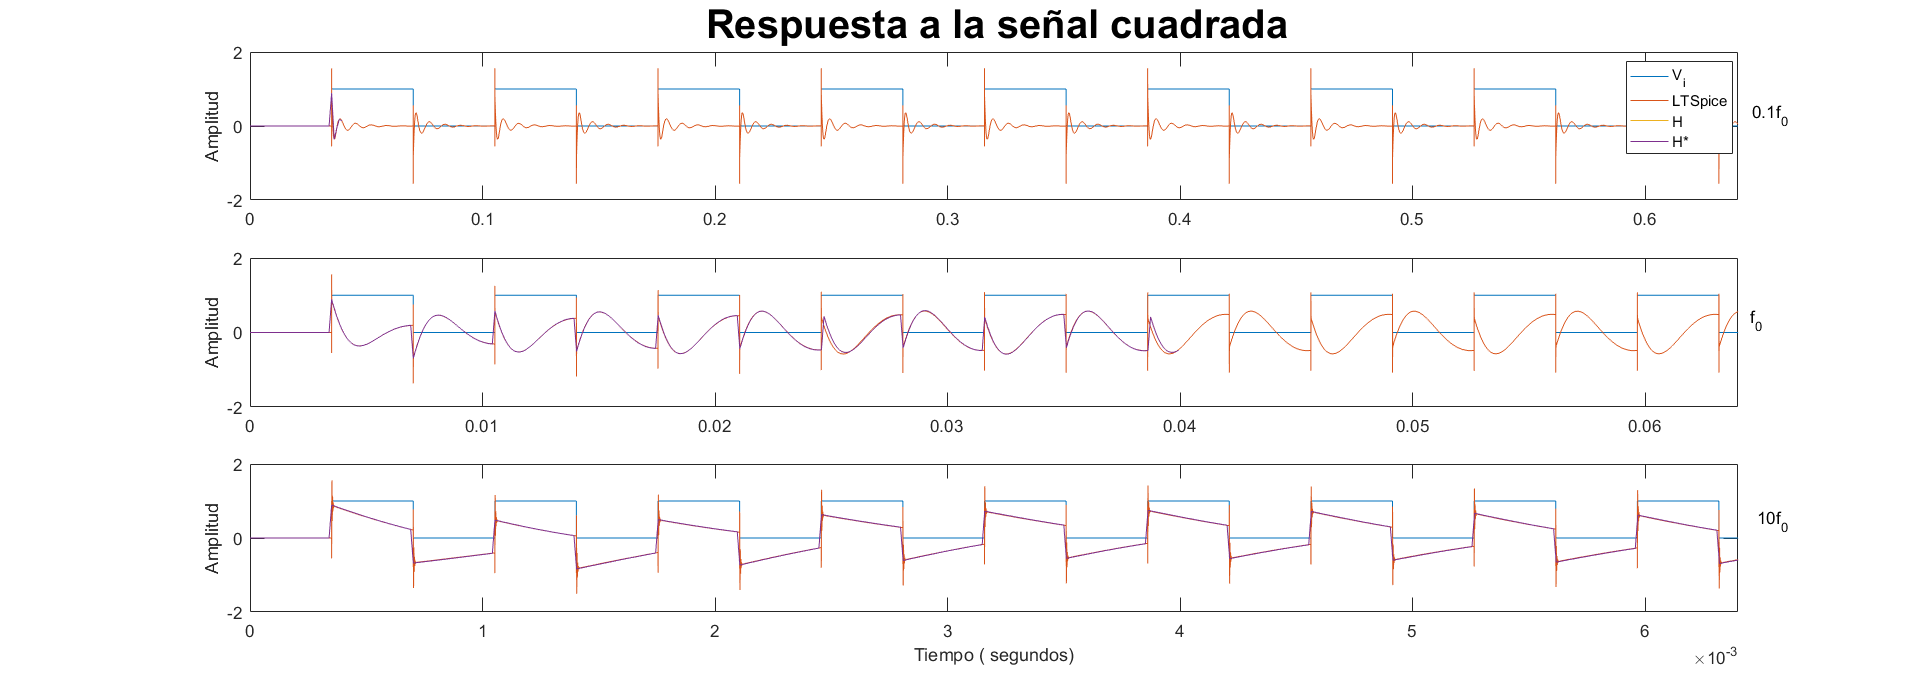
\includegraphics[width=1\textwidth]{resources/Comparacion_Cuadrada_LT.png}
    \caption{Respuesta a la cuadrada}
\end{figure}

Se puede observar que para los tres gráficos las señales de salida correspondientes a la simulación matemática y la simulación con LTSpice difieren relativamente poco. Sin embargo, la simulación de LTSpice presenta en todos los gŕaficos una diferencia en los primeros períodos  para luego estabilizarse a medida que transcurre el tiempo, estas diferencias podrían ser explicadas por las características internas del amplificador operacional.